% Options for packages loaded elsewhere
\PassOptionsToPackage{unicode}{hyperref}
\PassOptionsToPackage{hyphens}{url}
\PassOptionsToPackage{dvipsnames,svgnames,x11names}{xcolor}
%
\documentclass[
  12pt,
]{article}
\title{\hfill\break
\hfill\break
\hfill\break
\vspace{1cm}Customer dropout membership\footnote{Corresponding address: \href{mailto:sobreiro@esdrm.ipsantarem.pt}{\nolinkurl{sobreiro@esdrm.ipsantarem.pt}}. The current template adapts part of the Rmd code by \href{https://github.com/paulcbauer/Writing_a_reproducable_paper_in_rmarkdown}{Paul C. Bauer}, Mannheim Centre for European Social Research.}\vspace{0.5cm}}
\author{Pedro Sobreiro, Javier Berrocal, Domingos Martinho, José Garcia Alonso\\
~\\
Extremadura University\\}
\date{\hfill\break
\hfill\break
25 julho, 2021\\
~\\}

\usepackage{amsmath,amssymb}
\usepackage{lmodern}
\usepackage{setspace}
\usepackage{iftex}
\ifPDFTeX
  \usepackage[T1]{fontenc}
  \usepackage[utf8]{inputenc}
  \usepackage{textcomp} % provide euro and other symbols
\else % if luatex or xetex
  \usepackage{unicode-math}
  \defaultfontfeatures{Scale=MatchLowercase}
  \defaultfontfeatures[\rmfamily]{Ligatures=TeX,Scale=1}
  \setmainfont[]{Times New Roman}
  \setsansfont[]{Times New Roman}
\fi
% Use upquote if available, for straight quotes in verbatim environments
\IfFileExists{upquote.sty}{\usepackage{upquote}}{}
\IfFileExists{microtype.sty}{% use microtype if available
  \usepackage[]{microtype}
  \UseMicrotypeSet[protrusion]{basicmath} % disable protrusion for tt fonts
}{}
\makeatletter
\@ifundefined{KOMAClassName}{% if non-KOMA class
  \IfFileExists{parskip.sty}{%
    \usepackage{parskip}
  }{% else
    \setlength{\parindent}{0pt}
    \setlength{\parskip}{6pt plus 2pt minus 1pt}}
}{% if KOMA class
  \KOMAoptions{parskip=half}}
\makeatother
\usepackage{xcolor}
\IfFileExists{xurl.sty}{\usepackage{xurl}}{} % add URL line breaks if available
\IfFileExists{bookmark.sty}{\usepackage{bookmark}}{\usepackage{hyperref}}
\hypersetup{
  colorlinks=true,
  linkcolor={Maroon},
  filecolor={Maroon},
  citecolor={Blue},
  urlcolor={Blue},
  pdfcreator={LaTeX via pandoc}}
\urlstyle{same} % disable monospaced font for URLs
\usepackage[margin = 1in]{geometry}
\usepackage{color}
\usepackage{fancyvrb}
\newcommand{\VerbBar}{|}
\newcommand{\VERB}{\Verb[commandchars=\\\{\}]}
\DefineVerbatimEnvironment{Highlighting}{Verbatim}{commandchars=\\\{\}}
% Add ',fontsize=\small' for more characters per line
\usepackage{framed}
\definecolor{shadecolor}{RGB}{248,248,248}
\newenvironment{Shaded}{\begin{snugshade}}{\end{snugshade}}
\newcommand{\AlertTok}[1]{\textcolor[rgb]{0.94,0.16,0.16}{#1}}
\newcommand{\AnnotationTok}[1]{\textcolor[rgb]{0.56,0.35,0.01}{\textbf{\textit{#1}}}}
\newcommand{\AttributeTok}[1]{\textcolor[rgb]{0.77,0.63,0.00}{#1}}
\newcommand{\BaseNTok}[1]{\textcolor[rgb]{0.00,0.00,0.81}{#1}}
\newcommand{\BuiltInTok}[1]{#1}
\newcommand{\CharTok}[1]{\textcolor[rgb]{0.31,0.60,0.02}{#1}}
\newcommand{\CommentTok}[1]{\textcolor[rgb]{0.56,0.35,0.01}{\textit{#1}}}
\newcommand{\CommentVarTok}[1]{\textcolor[rgb]{0.56,0.35,0.01}{\textbf{\textit{#1}}}}
\newcommand{\ConstantTok}[1]{\textcolor[rgb]{0.00,0.00,0.00}{#1}}
\newcommand{\ControlFlowTok}[1]{\textcolor[rgb]{0.13,0.29,0.53}{\textbf{#1}}}
\newcommand{\DataTypeTok}[1]{\textcolor[rgb]{0.13,0.29,0.53}{#1}}
\newcommand{\DecValTok}[1]{\textcolor[rgb]{0.00,0.00,0.81}{#1}}
\newcommand{\DocumentationTok}[1]{\textcolor[rgb]{0.56,0.35,0.01}{\textbf{\textit{#1}}}}
\newcommand{\ErrorTok}[1]{\textcolor[rgb]{0.64,0.00,0.00}{\textbf{#1}}}
\newcommand{\ExtensionTok}[1]{#1}
\newcommand{\FloatTok}[1]{\textcolor[rgb]{0.00,0.00,0.81}{#1}}
\newcommand{\FunctionTok}[1]{\textcolor[rgb]{0.00,0.00,0.00}{#1}}
\newcommand{\ImportTok}[1]{#1}
\newcommand{\InformationTok}[1]{\textcolor[rgb]{0.56,0.35,0.01}{\textbf{\textit{#1}}}}
\newcommand{\KeywordTok}[1]{\textcolor[rgb]{0.13,0.29,0.53}{\textbf{#1}}}
\newcommand{\NormalTok}[1]{#1}
\newcommand{\OperatorTok}[1]{\textcolor[rgb]{0.81,0.36,0.00}{\textbf{#1}}}
\newcommand{\OtherTok}[1]{\textcolor[rgb]{0.56,0.35,0.01}{#1}}
\newcommand{\PreprocessorTok}[1]{\textcolor[rgb]{0.56,0.35,0.01}{\textit{#1}}}
\newcommand{\RegionMarkerTok}[1]{#1}
\newcommand{\SpecialCharTok}[1]{\textcolor[rgb]{0.00,0.00,0.00}{#1}}
\newcommand{\SpecialStringTok}[1]{\textcolor[rgb]{0.31,0.60,0.02}{#1}}
\newcommand{\StringTok}[1]{\textcolor[rgb]{0.31,0.60,0.02}{#1}}
\newcommand{\VariableTok}[1]{\textcolor[rgb]{0.00,0.00,0.00}{#1}}
\newcommand{\VerbatimStringTok}[1]{\textcolor[rgb]{0.31,0.60,0.02}{#1}}
\newcommand{\WarningTok}[1]{\textcolor[rgb]{0.56,0.35,0.01}{\textbf{\textit{#1}}}}
\usepackage{longtable,booktabs,array}
\usepackage{calc} % for calculating minipage widths
% Correct order of tables after \paragraph or \subparagraph
\usepackage{etoolbox}
\makeatletter
\patchcmd\longtable{\par}{\if@noskipsec\mbox{}\fi\par}{}{}
\makeatother
% Allow footnotes in longtable head/foot
\IfFileExists{footnotehyper.sty}{\usepackage{footnotehyper}}{\usepackage{footnote}}
\makesavenoteenv{longtable}
\usepackage{graphicx}
\makeatletter
\def\maxwidth{\ifdim\Gin@nat@width>\linewidth\linewidth\else\Gin@nat@width\fi}
\def\maxheight{\ifdim\Gin@nat@height>\textheight\textheight\else\Gin@nat@height\fi}
\makeatother
% Scale images if necessary, so that they will not overflow the page
% margins by default, and it is still possible to overwrite the defaults
% using explicit options in \includegraphics[width, height, ...]{}
\setkeys{Gin}{width=\maxwidth,height=\maxheight,keepaspectratio}
% Set default figure placement to htbp
\makeatletter
\def\fps@figure{htbp}
\makeatother
\setlength{\emergencystretch}{3em} % prevent overfull lines
\providecommand{\tightlist}{%
  \setlength{\itemsep}{0pt}\setlength{\parskip}{0pt}}
\setcounter{secnumdepth}{5}
\newlength{\cslhangindent}
\setlength{\cslhangindent}{1.5em}
\newlength{\csllabelwidth}
\setlength{\csllabelwidth}{3em}
\newlength{\cslentryspacingunit} % times entry-spacing
\setlength{\cslentryspacingunit}{\parskip}
\newenvironment{CSLReferences}[2] % #1 hanging-ident, #2 entry spacing
 {% don't indent paragraphs
  \setlength{\parindent}{0pt}
  % turn on hanging indent if param 1 is 1
  \ifodd #1
  \let\oldpar\par
  \def\par{\hangindent=\cslhangindent\oldpar}
  \fi
  % set entry spacing
  \setlength{\parskip}{#2\cslentryspacingunit}
 }%
 {}
\usepackage{calc}
\newcommand{\CSLBlock}[1]{#1\hfill\break}
\newcommand{\CSLLeftMargin}[1]{\parbox[t]{\csllabelwidth}{#1}}
\newcommand{\CSLRightInline}[1]{\parbox[t]{\linewidth - \csllabelwidth}{#1}\break}
\newcommand{\CSLIndent}[1]{\hspace{\cslhangindent}#1}
\usepackage{dcolumn}
\usepackage{color}
\usepackage{pdfpages}
\usepackage{amsmath}
\usepackage{booktabs}
\usepackage{makecell}
\usepackage{hyperref}
\usepackage{booktabs}
\usepackage{longtable}
\usepackage{array}
\usepackage{multirow}
\usepackage{wrapfig}
\usepackage{float}
\usepackage{colortbl}
\usepackage{pdflscape}
\usepackage{tabu}
\usepackage{threeparttable}
\usepackage{threeparttablex}
\usepackage[normalem]{ulem}
\usepackage{makecell}
\usepackage{xcolor}
\ifLuaTeX
  \usepackage{selnolig}  % disable illegal ligatures
\fi

\begin{document}
\maketitle
\begin{abstract}
\noindent\setstretch{1}Abstract of the article. Here we can place more info.\vspace{.8cm}
\end{abstract}

\setstretch{1.2}
\hypertarget{introduction}{%
\section{Introduction}\label{introduction}}

Research idea:

\begin{itemize}
\tightlist
\item
\end{itemize}

Context: An organization membership located in Portugal. The organization offers
an annual membership for the members, the service subscription has several
payment options:

\begin{itemize}
\tightlist
\item
  Men with a annual fee of 10€
\item
  Women annual fee of 6€
\item
  Correspondent fee 6€
\item
  Retired fee 5€
\item
  Student fee 2.5€
\item
  under-14 fee 1€
\end{itemize}

\clearpage

\renewcommand{\baselinestretch}{0.5}\normalsize

\renewcommand{\baselinestretch}{1.1}\normalsize

\clearpage

\begin{Shaded}
\begin{Highlighting}[]
\FunctionTok{library}\NormalTok{(dplyr)}
\FunctionTok{library}\NormalTok{(dlookr)}
\FunctionTok{library}\NormalTok{(ggplot2)}

\CommentTok{\#eda\_report(nlswork,output\_dir  = }
\CommentTok{\#   "C:/Users/mangelo.EEG/Documents/GitHub/prjs/reports/",}
\CommentTok{\#   output\_file = "eda\_report.pdf")}

\DocumentationTok{\#\# The data}

\FunctionTok{names}\NormalTok{(airquality)}
\end{Highlighting}
\end{Shaded}

\begin{verbatim}
## [1] "Ozone"   "Solar.R" "Wind"    "Temp"    "Month"   "Day"
\end{verbatim}

\begin{Shaded}
\begin{Highlighting}[]
\CommentTok{\#summary(nlswork)}

\DocumentationTok{\#\# Missing values}
\FunctionTok{library}\NormalTok{(visdat)}
\FunctionTok{vis\_dat}\NormalTok{(airquality)}
\end{Highlighting}
\end{Shaded}

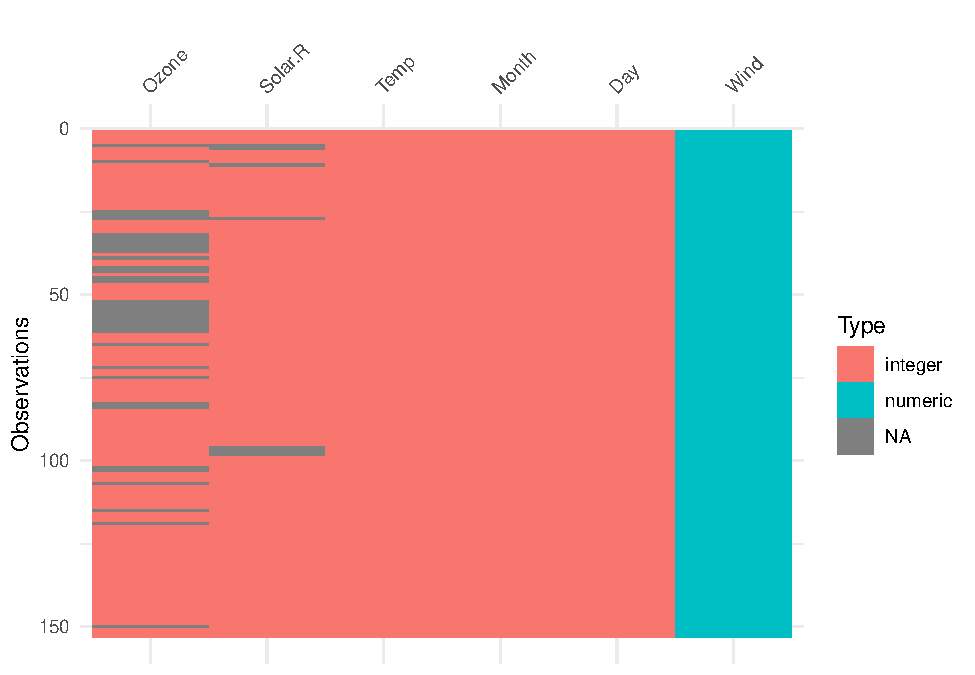
\includegraphics{articleCustomerDropoutMembership_files/figure-latex/Stats1-1.pdf}

\begin{Shaded}
\begin{Highlighting}[]
\FunctionTok{library}\NormalTok{(naniar)}
\FunctionTok{vis\_miss}\NormalTok{(airquality)}
\end{Highlighting}
\end{Shaded}

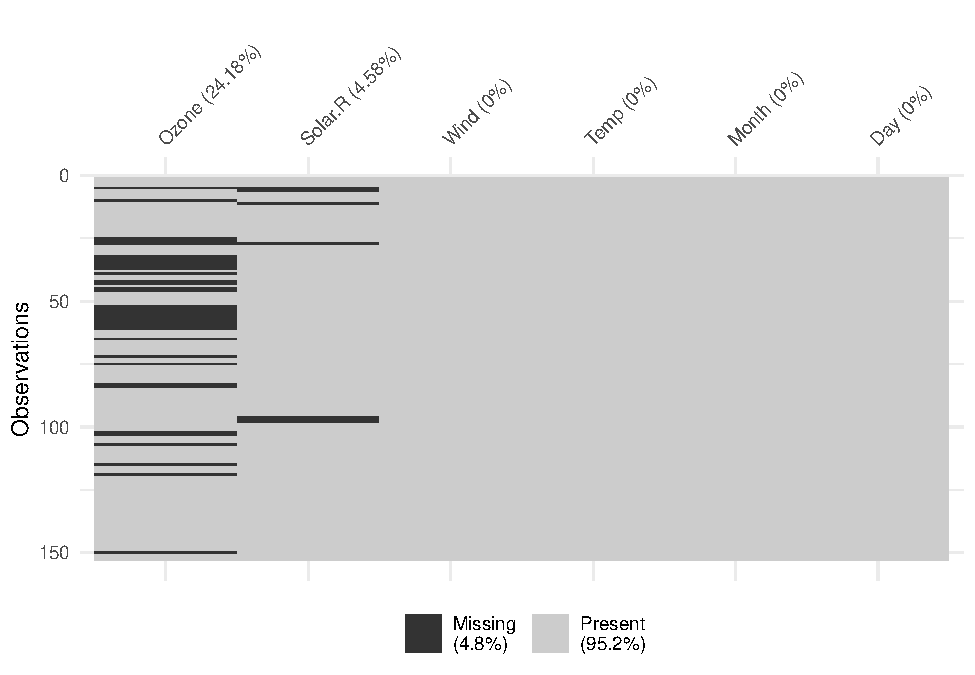
\includegraphics{articleCustomerDropoutMembership_files/figure-latex/Stats1-2.pdf}

\begin{Shaded}
\begin{Highlighting}[]
\FunctionTok{gg\_miss\_upset}\NormalTok{(airquality)}
\end{Highlighting}
\end{Shaded}

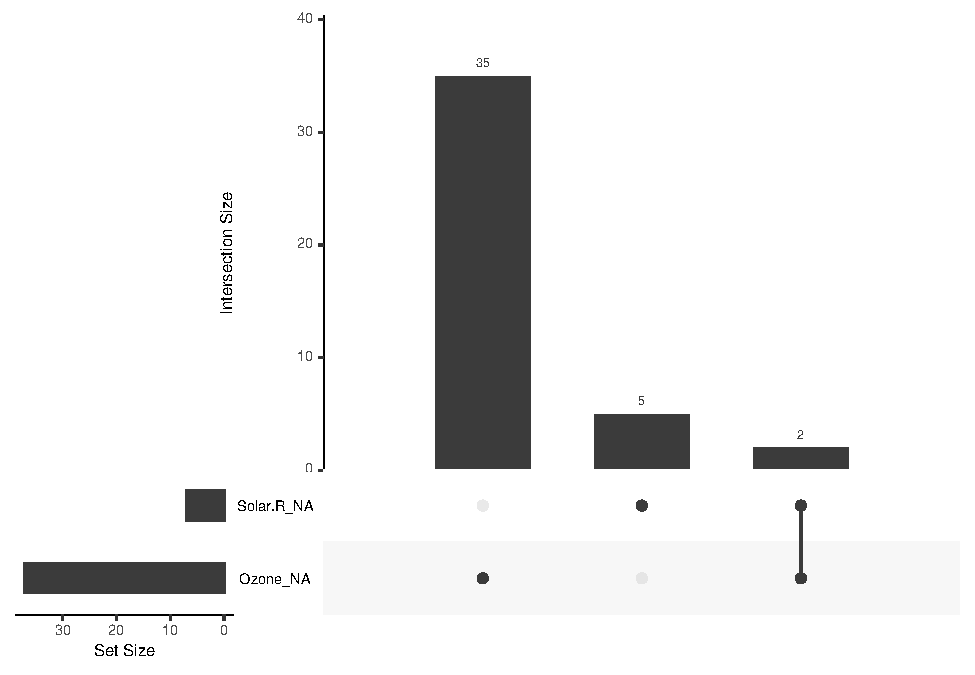
\includegraphics{articleCustomerDropoutMembership_files/figure-latex/Stats1-3.pdf}

\begin{Shaded}
\begin{Highlighting}[]
\DocumentationTok{\#\# GRAPHS}
\NormalTok{dplyr}\SpecialCharTok{::}\FunctionTok{glimpse}\NormalTok{(cars}\SpecialCharTok{$}\NormalTok{Ozone)}
\end{Highlighting}
\end{Shaded}

\begin{verbatim}
##  NULL
\end{verbatim}

\begin{Shaded}
\begin{Highlighting}[]
\NormalTok{d }\OtherTok{\textless{}{-}} \FunctionTok{density}\NormalTok{(airquality}\SpecialCharTok{$}\NormalTok{Temp)}
\FunctionTok{plot}\NormalTok{(d)}
\end{Highlighting}
\end{Shaded}

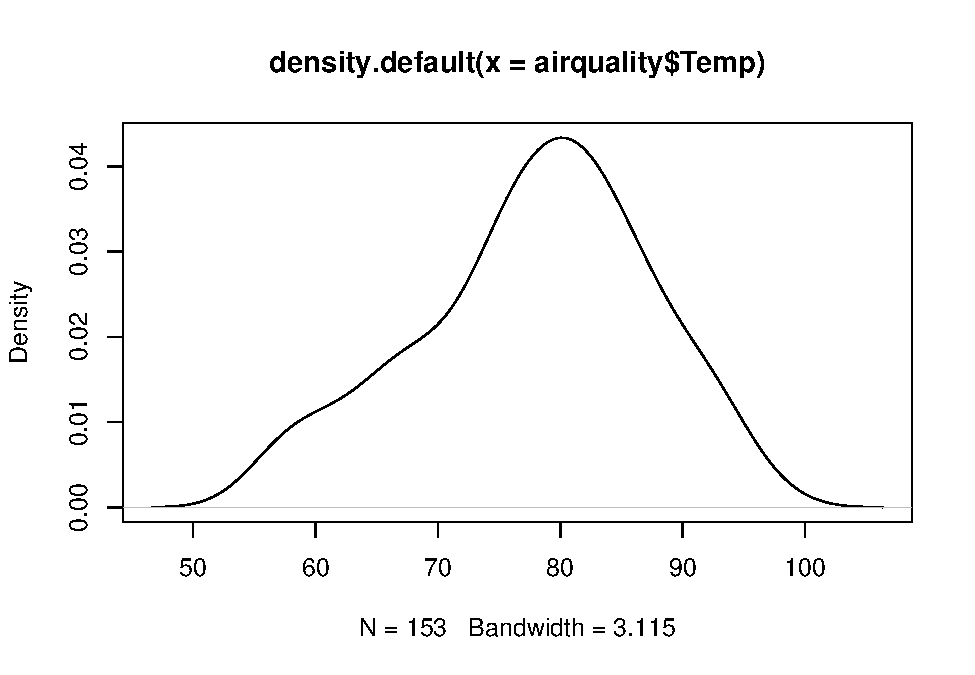
\includegraphics{articleCustomerDropoutMembership_files/figure-latex/Stats1-4.pdf}

\begin{Shaded}
\begin{Highlighting}[]
\FunctionTok{plot}\NormalTok{(airquality}\SpecialCharTok{$}\NormalTok{Ozone, airquality}\SpecialCharTok{$}\NormalTok{Solar.R)}
\end{Highlighting}
\end{Shaded}

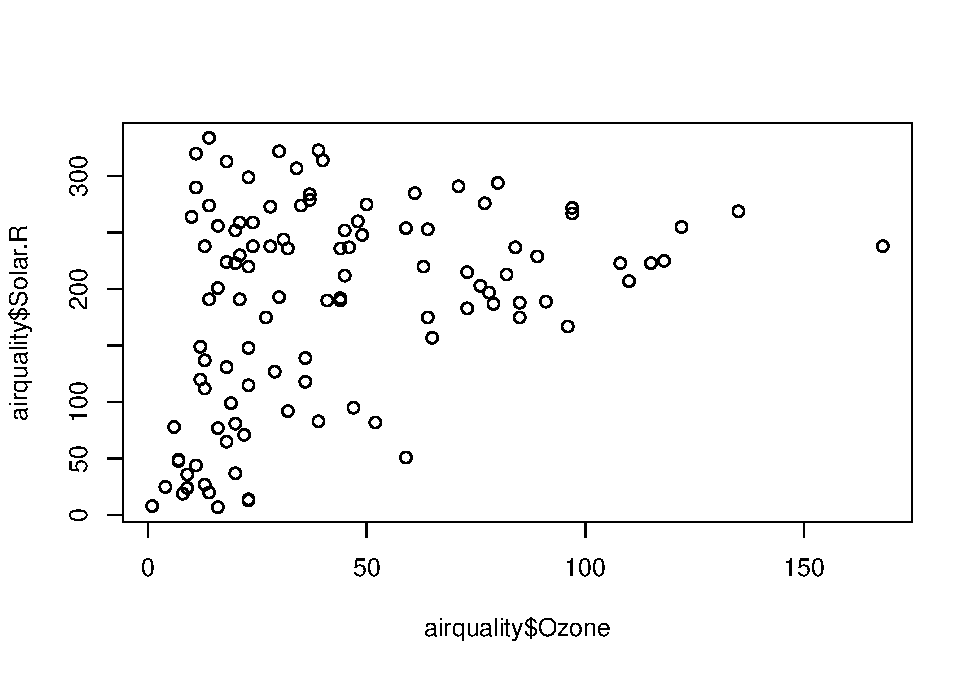
\includegraphics{articleCustomerDropoutMembership_files/figure-latex/Stats1-5.pdf}

\begin{Shaded}
\begin{Highlighting}[]
\FunctionTok{ggplot}\NormalTok{(airquality, }\FunctionTok{aes}\NormalTok{(}\AttributeTok{x =}\NormalTok{ Ozone, }\AttributeTok{y =}\NormalTok{ Solar.R)) }\SpecialCharTok{+}
\FunctionTok{geom\_miss\_point}\NormalTok{()}
\end{Highlighting}
\end{Shaded}

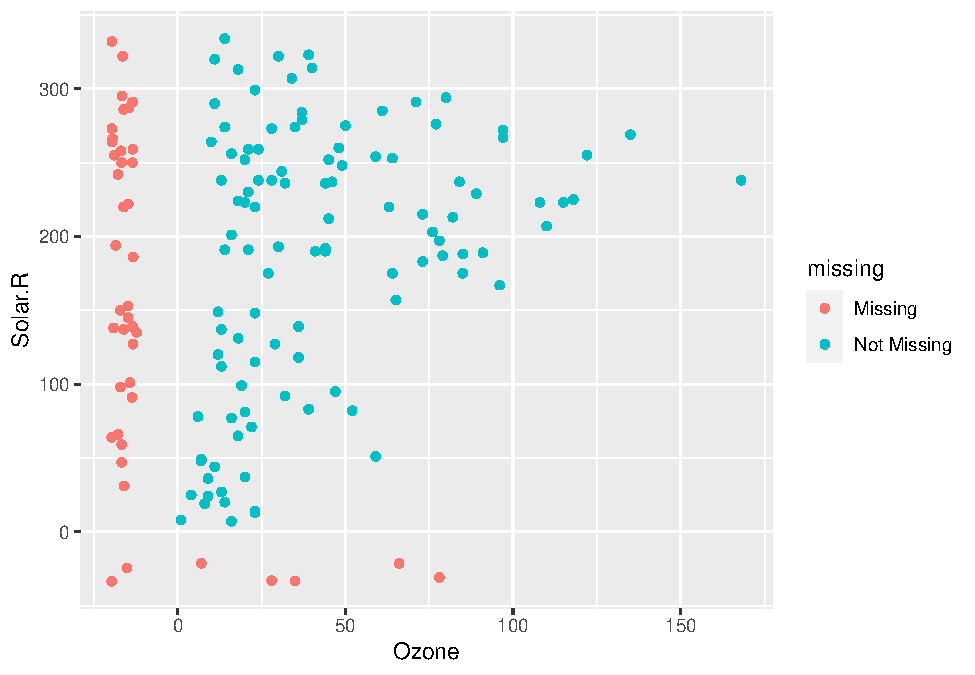
\includegraphics{articleCustomerDropoutMembership_files/figure-latex/Stats1-6.pdf}

\begin{Shaded}
\begin{Highlighting}[]
\FunctionTok{ggplot}\NormalTok{(airquality, }\FunctionTok{aes}\NormalTok{(}\AttributeTok{x =}\NormalTok{ Wind, }\AttributeTok{y =}\NormalTok{ Temp)) }\SpecialCharTok{+}
\FunctionTok{geom\_miss\_point}\NormalTok{() }\SpecialCharTok{+}
\FunctionTok{facet\_wrap}\NormalTok{(}\FunctionTok{vars}\NormalTok{(Month))}
\end{Highlighting}
\end{Shaded}

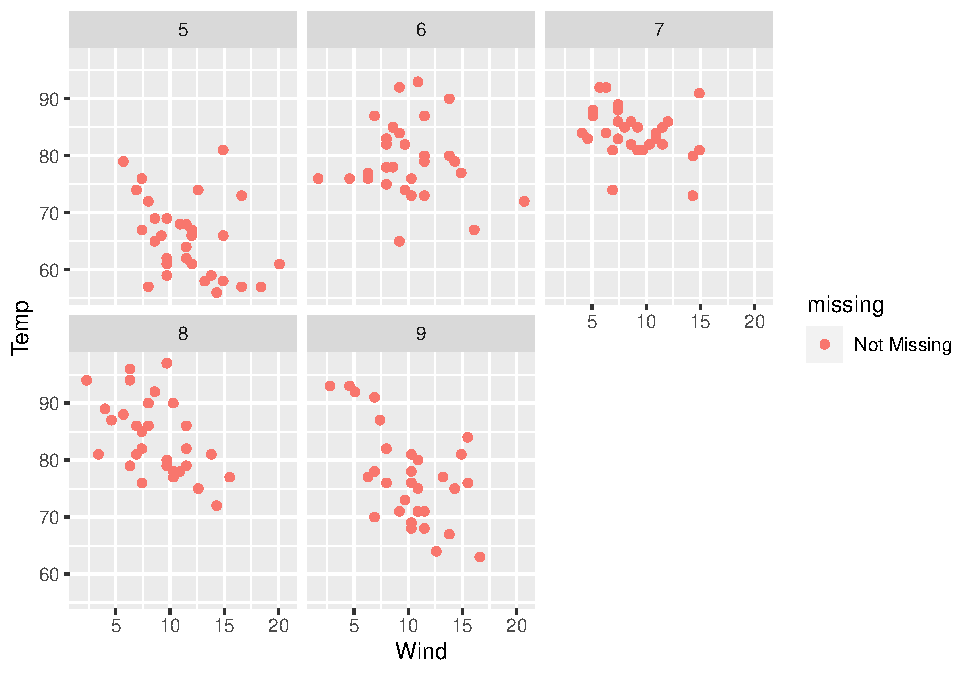
\includegraphics{articleCustomerDropoutMembership_files/figure-latex/Stats1-7.pdf}

\begin{Shaded}
\begin{Highlighting}[]
\NormalTok{stats }\OtherTok{\textless{}{-}} \FunctionTok{summary}\NormalTok{(airquality}\SpecialCharTok{$}\NormalTok{Temp)}
\NormalTok{stats}
\end{Highlighting}
\end{Shaded}

\begin{verbatim}
##    Min. 1st Qu.  Median    Mean 3rd Qu.    Max. 
##   56.00   72.00   79.00   77.88   85.00   97.00
\end{verbatim}

\begin{Shaded}
\begin{Highlighting}[]
\FunctionTok{describe}\NormalTok{(airquality)}
\end{Highlighting}
\end{Shaded}

\begin{verbatim}
## # A tibble: 6 x 26
##   variable     n    na   mean    sd se_mean   IQR skewness kurtosis   p00   p01
##   <chr>    <int> <int>  <dbl> <dbl>   <dbl> <dbl>    <dbl>    <dbl> <dbl> <dbl>
## 1 Ozone      116    37  42.1  33.0    3.06   45.2  1.24       1.29    1    4.3 
## 2 Solar.R    146     7 186.   90.1    7.45  143   -0.428     -0.968   7   10.2 
## 3 Wind       153     0   9.96  3.52   0.285   4.1  0.348      0.111   1.7  2.56
## 4 Temp       153     0  77.9   9.47   0.765  13   -0.378     -0.404  56   57   
## 5 Month      153     0   6.99  1.42   0.115   2   -0.00239   -1.30    5    5   
## 6 Day        153     0  15.8   8.86   0.717  15    0.00265   -1.20    1    1   
## # ... with 15 more variables: p05 <dbl>, p10 <dbl>, p20 <dbl>, p25 <dbl>,
## #   p30 <dbl>, p40 <dbl>, p50 <dbl>, p60 <dbl>, p70 <dbl>, p75 <dbl>,
## #   p80 <dbl>, p90 <dbl>, p95 <dbl>, p99 <dbl>, p100 <dbl>
\end{verbatim}

\hypertarget{experimental-results}{%
\section{Experimental Results}\label{experimental-results}}

\hypertarget{data-description}{%
\subsection{Data description}\label{data-description}}

\begin{verbatim}
##  [1] "Sócio"               "dataAdesao"          "ano"                
##  [4] "dataNascimento"      "idade"               "sexo"               
##  [7] "estadoCivil"         "categoria"           "quotaMensal"        
## [10] "profissao"           "codPostal"           "ultimaQuota"        
## [13] "ultimoPagamento"     "valorTotal"          "totalJogos"         
## [16] "jogosEpoca"          "diasUltimoPagamento" "mesesUP"            
## [19] "abandonou"           "anosSocio"           "idaEstadio"         
## [22] "escaloesTotalJogos"  "mes"
\end{verbatim}

\begin{verbatim}
##  [1] "num_socio"                 "dt_inscription"           
##  [3] "year"                      "birth_date"               
##  [5] "age"                       "sex"                      
##  [7] "marital_status"            "category"                 
##  [9] "monthly_fee"               "occupation"               
## [11] "zip_code"                  "dt_last_invoice"          
## [13] "dt_last_payment"           "total_amount"             
## [15] "total_matches"             "season_matches"           
## [17] "days_since_last_payment"   "months_since_last_payment"
## [19] "dropout"                   "years_membership"         
## [21] "stadium_access"            "quart_stadium_entries"    
## [23] "inscription_month"
\end{verbatim}

\begin{verbatim}
## tibble [25,316 x 14] (S3: tbl_df/tbl/data.frame)
##  $ year                     : num [1:25316] 1944 1944 1945 1945 1945 ...
##  $ age                      : num [1:25316] 83 88 73 97 97 91 88 95 88 78 ...
##  $ sex                      : chr [1:25316] "M" "M" "M" "M" ...
##  $ marital_status           : chr [1:25316] "casado" "solteiro" "nao definido" "casado" ...
##  $ monthly_fee              : num [1:25316] 10 10 10 5 10 5 5 5 10 10 ...
##  $ total_amount             : num [1:25316] 1906 1906 1553 790 1466 ...
##  $ total_matches            : num [1:25316] 0 0 0 0 0 20 74 0 154 0 ...
##  $ season_matches           : num [1:25316] 0 0 0 0 0 0 0 0 6 0 ...
##  $ months_since_last_payment: num [1:25316] 3 3 36 8 35 4 41 40 4 2 ...
##  $ dropout                  : num [1:25316] 0 0 1 0 1 0 1 1 0 0 ...
##  $ years_membership         : num [1:25316] 74 74 73 73 73 73 73 73 73 72 ...
##  $ stadium_access           : num [1:25316] 0 0 0 0 0 1 1 0 1 0 ...
##  $ quart_stadium_entries    : chr [1:25316] "ate 1" "ate 1" "ate 1" "ate 1" ...
##  $ inscription_month        : num [1:25316] 10 10 8 9 9 12 1 1 2 4 ...
\end{verbatim}

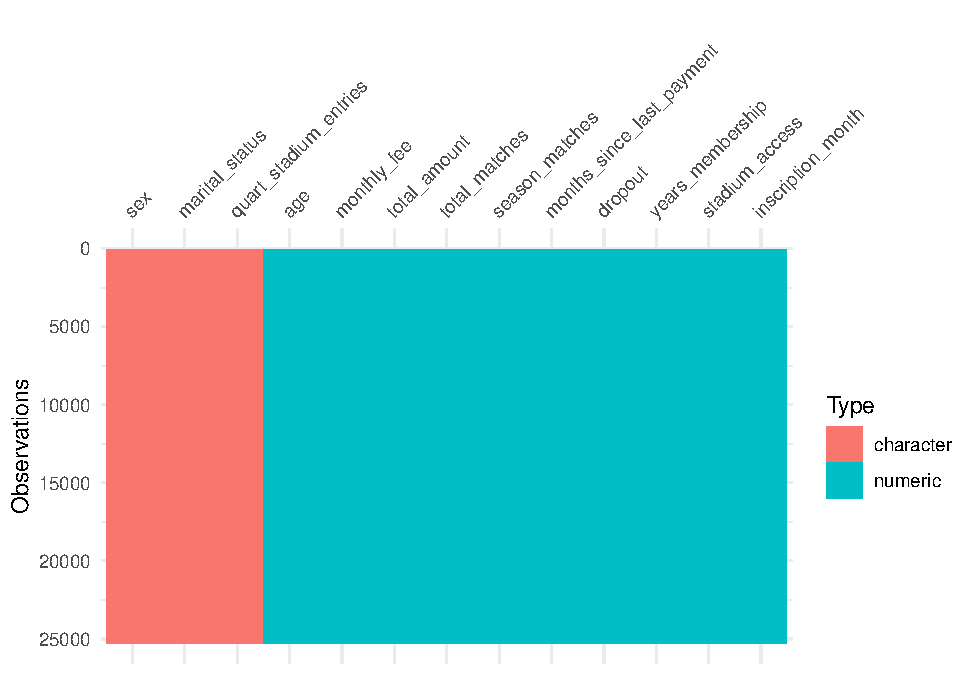
\includegraphics{articleCustomerDropoutMembership_files/figure-latex/get_data-1.pdf}

Table \ref{tab:tab1cars} shows data's summary statistics.\footnote{You can reference the table as \ref{tab1cars}.} \texttt{stargazer()} is
and excellent solution to export outputs.

Teste \ref{tab:summarytable}

\begin{table}

\caption{\label{tab:summarytable}Summary statistics}
\centering
\begin{tabular}[t]{ll}
\toprule
Characteristic & N = 25,316\\
\midrule
year & 2,007 (11)\\
age & 27 (20)\\
sex & \\
\hspace{1em}F & 32\%\\
\hspace{1em}M & 68\%\\
\addlinespace
marital\_status & \\
\hspace{1em}casado & 20\%\\
\hspace{1em}nao definido & 30\%\\
\hspace{1em}outro & 2.0\%\\
\hspace{1em}solteiro & 48\%\\
\addlinespace
monthly\_fee & \\
\hspace{1em}0 & <0.1\%\\
\hspace{1em}1 & 32\%\\
\hspace{1em}2.5 & 28\%\\
\hspace{1em}5 & 3.4\%\\
\addlinespace
\hspace{1em}6 & 12\%\\
\hspace{1em}10 & 24\%\\
total\_amount & 316 (494)\\
total\_matches & 27 (46)\\
season\_matches & 2.2 (4.1)\\
\addlinespace
months\_since\_last\_payment & 19 (32)\\
dropout & 22\%\\
years\_membership & 11 (11)\\
stadium\_access & 40\%\\
quart\_stadium\_entries & \\
\addlinespace
\hspace{1em}1 a 21 & 10\%\\
\hspace{1em}21 a 56 & 9.8\%\\
\hspace{1em}56 a 105 & 10.0\%\\
\hspace{1em}ate 1 & 60\%\\
\hspace{1em}mais 105 & 10.0\%\\
\addlinespace
inscription\_month & 6.9 (3.4)\\
\bottomrule
\multicolumn{2}{l}{\rule{0pt}{1em}\textsuperscript{1} Mean (SD); \%}\\
\end{tabular}
\end{table}

\begin{Shaded}
\begin{Highlighting}[]
\CommentTok{\#from pysurvival.utils.display import correlation\_matrix}
\ImportTok{import}\NormalTok{ pandas }\ImportTok{as}\NormalTok{ pd}
\ImportTok{import}\NormalTok{ numpy }\ImportTok{as}\NormalTok{ np}

\NormalTok{col }\OperatorTok{=}\NormalTok{ [}\StringTok{\textquotesingle{}sex\textquotesingle{}}\NormalTok{,}\StringTok{\textquotesingle{}marital\_status\textquotesingle{}}\NormalTok{,}\StringTok{\textquotesingle{}quart\_stadium\_entries\textquotesingle{}}\NormalTok{]}

\NormalTok{df\_members }\OperatorTok{=}\NormalTok{ r.df\_members }\CommentTok{\#copy r dataframe to python}

\NormalTok{df\_members }\OperatorTok{=}\NormalTok{ pd.get\_dummies(df\_members, columns}\OperatorTok{=}\NormalTok{col,drop\_first}\OperatorTok{=}\VariableTok{True}\NormalTok{)}

\CommentTok{\# Creating the time and event columns}
\NormalTok{time\_column }\OperatorTok{=} \StringTok{\textquotesingle{}years\_membership\textquotesingle{}}
\NormalTok{event\_column }\OperatorTok{=} \StringTok{\textquotesingle{}dropout\textquotesingle{}}

\CommentTok{\# Extracting the features}
\NormalTok{features }\OperatorTok{=}\NormalTok{ np.setdiff1d(df\_members.columns, [time\_column, event\_column] ).tolist()}


\CommentTok{\#correlation\_matrix(df\_members, figure\_size=(10,10), text\_fontsize=6)}
\end{Highlighting}
\end{Shaded}

The average age in our data is 27.3.

\hypertarget{sec:tables}{%
\section{Tables}\label{sec:tables}}

R Markdown PDF is now able to produce good tables with our output. For
\texttt{stargazer} the label is contained in the function, while for \texttt{kable} it's
contained in the chunk name.

\hypertarget{stargazer-summary-and-regression-tables}{%
\subsection{stargazer(): Summary and regression tables}\label{stargazer-summary-and-regression-tables}}

Table \ref{tab2} reports regression outputs. Name the models as you can refer
to their names in the text (M1, M2, M3).

\begin{Shaded}
\begin{Highlighting}[]
\FunctionTok{library}\NormalTok{(stargazer)}
\NormalTok{model1 }\OtherTok{\textless{}{-}} \FunctionTok{lm}\NormalTok{(speed }\SpecialCharTok{\textasciitilde{}}\NormalTok{ dist, }\AttributeTok{data =}\NormalTok{ cars)}
\NormalTok{model2 }\OtherTok{\textless{}{-}} \FunctionTok{lm}\NormalTok{(speed }\SpecialCharTok{\textasciitilde{}}\NormalTok{ dist, }\AttributeTok{data =}\NormalTok{ cars)}
\NormalTok{model3 }\OtherTok{\textless{}{-}} \FunctionTok{lm}\NormalTok{(dist }\SpecialCharTok{\textasciitilde{}}\NormalTok{ speed, }\AttributeTok{data =}\NormalTok{ cars)}
\FunctionTok{stargazer}\NormalTok{(model1, model2, model3,}
          \AttributeTok{title =} \StringTok{"Regression table with stargazer"}\NormalTok{,}
          \AttributeTok{label =} \StringTok{"tab2"}\NormalTok{,}
          \AttributeTok{table.placement =} \StringTok{"h"}\NormalTok{,}
          \AttributeTok{column.labels =} \FunctionTok{c}\NormalTok{(}\StringTok{"M1"}\NormalTok{, }\StringTok{"M2"}\NormalTok{, }\StringTok{"M3"}\NormalTok{),}
          \AttributeTok{model.numbers =} \ConstantTok{FALSE}\NormalTok{,}
          \AttributeTok{header =} \ConstantTok{FALSE}\NormalTok{)}
\end{Highlighting}
\end{Shaded}

\begin{table}[h] \centering 
  \caption{Regression table with stargazer} 
  \label{tab2} 
\begin{tabular}{@{\extracolsep{5pt}}lccc} 
\\[-1.8ex]\hline 
\hline \\[-1.8ex] 
 & \multicolumn{3}{c}{\textit{Dependent variable:}} \\ 
\cline{2-4} 
\\[-1.8ex] & \multicolumn{2}{c}{speed} & dist \\ 
 & M1 & M2 & M3 \\ 
\hline \\[-1.8ex] 
 dist & 0.166$^{***}$ & 0.166$^{***}$ &  \\ 
  & (0.017) & (0.017) &  \\ 
  & & & \\ 
 speed &  &  & 3.932$^{***}$ \\ 
  &  &  & (0.416) \\ 
  & & & \\ 
 Constant & 8.284$^{***}$ & 8.284$^{***}$ & $-$17.579$^{**}$ \\ 
  & (0.874) & (0.874) & (6.758) \\ 
  & & & \\ 
\hline \\[-1.8ex] 
Observations & 50 & 50 & 50 \\ 
R$^{2}$ & 0.651 & 0.651 & 0.651 \\ 
Adjusted R$^{2}$ & 0.644 & 0.644 & 0.644 \\ 
Residual Std. Error (df = 48) & 3.156 & 3.156 & 15.380 \\ 
F Statistic (df = 1; 48) & 89.567$^{***}$ & 89.567$^{***}$ & 89.567$^{***}$ \\ 
\hline 
\hline \\[-1.8ex] 
\textit{Note:}  & \multicolumn{3}{r}{$^{*}$p$<$0.1; $^{**}$p$<$0.05; $^{***}$p$<$0.01} \\ 
\end{tabular} 
\end{table}

\hypertarget{figures}{%
\section{Figures}\label{figures}}

\hypertarget{graphs-with-r}{%
\subsection{Graphs with R}\label{graphs-with-r}}

You can insert figures like this. One would like to produce and insert them on
the fly in the \texttt{.rmd} file. Figure \ref{fig:fig-1} is such an example.

\begin{Shaded}
\begin{Highlighting}[]
\FunctionTok{plot}\NormalTok{(cars}\SpecialCharTok{$}\NormalTok{speed, cars}\SpecialCharTok{$}\NormalTok{dist)}
\end{Highlighting}
\end{Shaded}

\begin{figure}[h]

{\centering 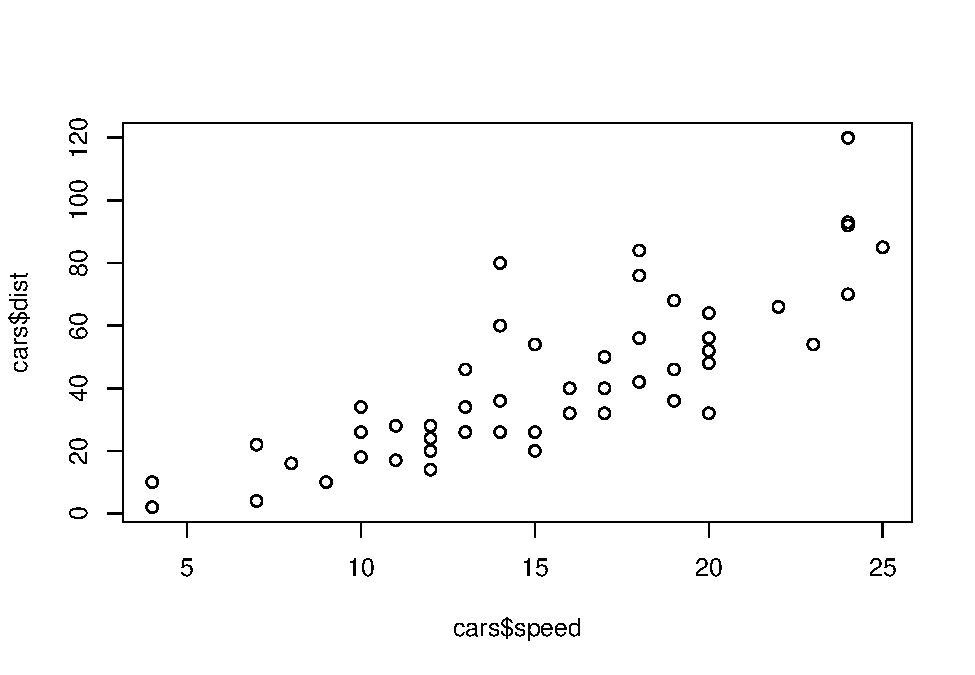
\includegraphics{articleCustomerDropoutMembership_files/figure-latex/Figures 1, fig-1-1} 

}

\caption{Scatterplot of Speed and Distance}(\#fig:Figures 1, fig-1)
\end{figure}

However, in some cases it does not work.

\hypertarget{example-ggplot2-graphs}{%
\subsection{Example: ggplot2 graphs}\label{example-ggplot2-graphs}}

See the \texttt{ggplot2} output reported in Figure \ref{fig:fig-2}.

\begin{Shaded}
\begin{Highlighting}[]
\NormalTok{mtcars}\SpecialCharTok{$}\NormalTok{cyl }\OtherTok{\textless{}{-}} \FunctionTok{as.factor}\NormalTok{(mtcars}\SpecialCharTok{$}\NormalTok{cyl) }\CommentTok{\# Convert cyl to factor}
\FunctionTok{library}\NormalTok{(ggplot2)}
\FunctionTok{ggplot}\NormalTok{(mtcars, }\FunctionTok{aes}\NormalTok{(}\AttributeTok{x =}\NormalTok{ wt, }\AttributeTok{y =}\NormalTok{ mpg, }\AttributeTok{shape =}\NormalTok{ cyl)) }\SpecialCharTok{+} \FunctionTok{geom\_point}\NormalTok{() }\SpecialCharTok{+}
  \FunctionTok{labs}\NormalTok{(}\AttributeTok{x =} \StringTok{"Weight (lb/1000)"}\NormalTok{, }\AttributeTok{y =} \StringTok{"Miles/(US) gallon"}\NormalTok{,}
       \AttributeTok{shape =} \StringTok{"Number of }\SpecialCharTok{\textbackslash{}n}\StringTok{ Cylinders"}\NormalTok{) }\SpecialCharTok{+} \FunctionTok{theme\_classic}\NormalTok{()}
\end{Highlighting}
\end{Shaded}

\begin{figure}[h]

{\centering 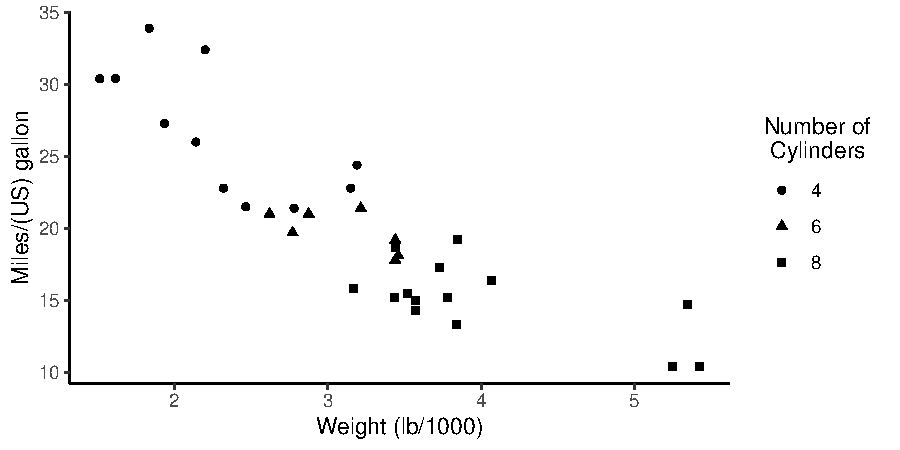
\includegraphics{articleCustomerDropoutMembership_files/figure-latex/Fig-2-1} 

}

\caption{Miles per gallon according to the weight}\label{fig:Fig-2}
\end{figure}

\hypertarget{another-example-using-plotly}{%
\subsection{Another example using Plotly}\label{another-example-using-plotly}}

With \texttt{Plotly} we can produce interactive graphs which play well, for example,
once can embedded in html webpages (drop by
\href{https://paulcbauer.shinyapps.io/visualizing-causal-scenarios/}{here} for an
example). One can insert this type of graphs in R Markdown PDF using \texttt{Orca} (it
generates static images from Plotly graphs). Go
\href{https://github.com/plotly/orca\#installation}{here} to check how to install it.
See Figure \ref{fig:fig-3} for an example.

\begin{Shaded}
\begin{Highlighting}[]
\FunctionTok{library}\NormalTok{(plotly)}
\NormalTok{p }\OtherTok{\textless{}{-}} \FunctionTok{plot\_ly}\NormalTok{(cars, }\AttributeTok{type =} \StringTok{"scatter"}\NormalTok{, }\AttributeTok{mode =} \StringTok{"markers"}\NormalTok{,}
        \AttributeTok{x =} \SpecialCharTok{\textasciitilde{}}\NormalTok{speed,}
        \AttributeTok{y =} \SpecialCharTok{\textasciitilde{}}\NormalTok{dist)}
\CommentTok{\#Sys.setenv(\textquotesingle{}MAPBOX\_TOKEN\textquotesingle{} = \textquotesingle{}12423423\textquotesingle{}) \# set arbitrary token}
\CommentTok{\#orca(p, "logs/plotly{-}plot.pdf")}
\end{Highlighting}
\end{Shaded}

\begin{figure}[ht]
\centering
\caption{Example: export a Plotly figure using `orca`}\label{fig:fig-3}
    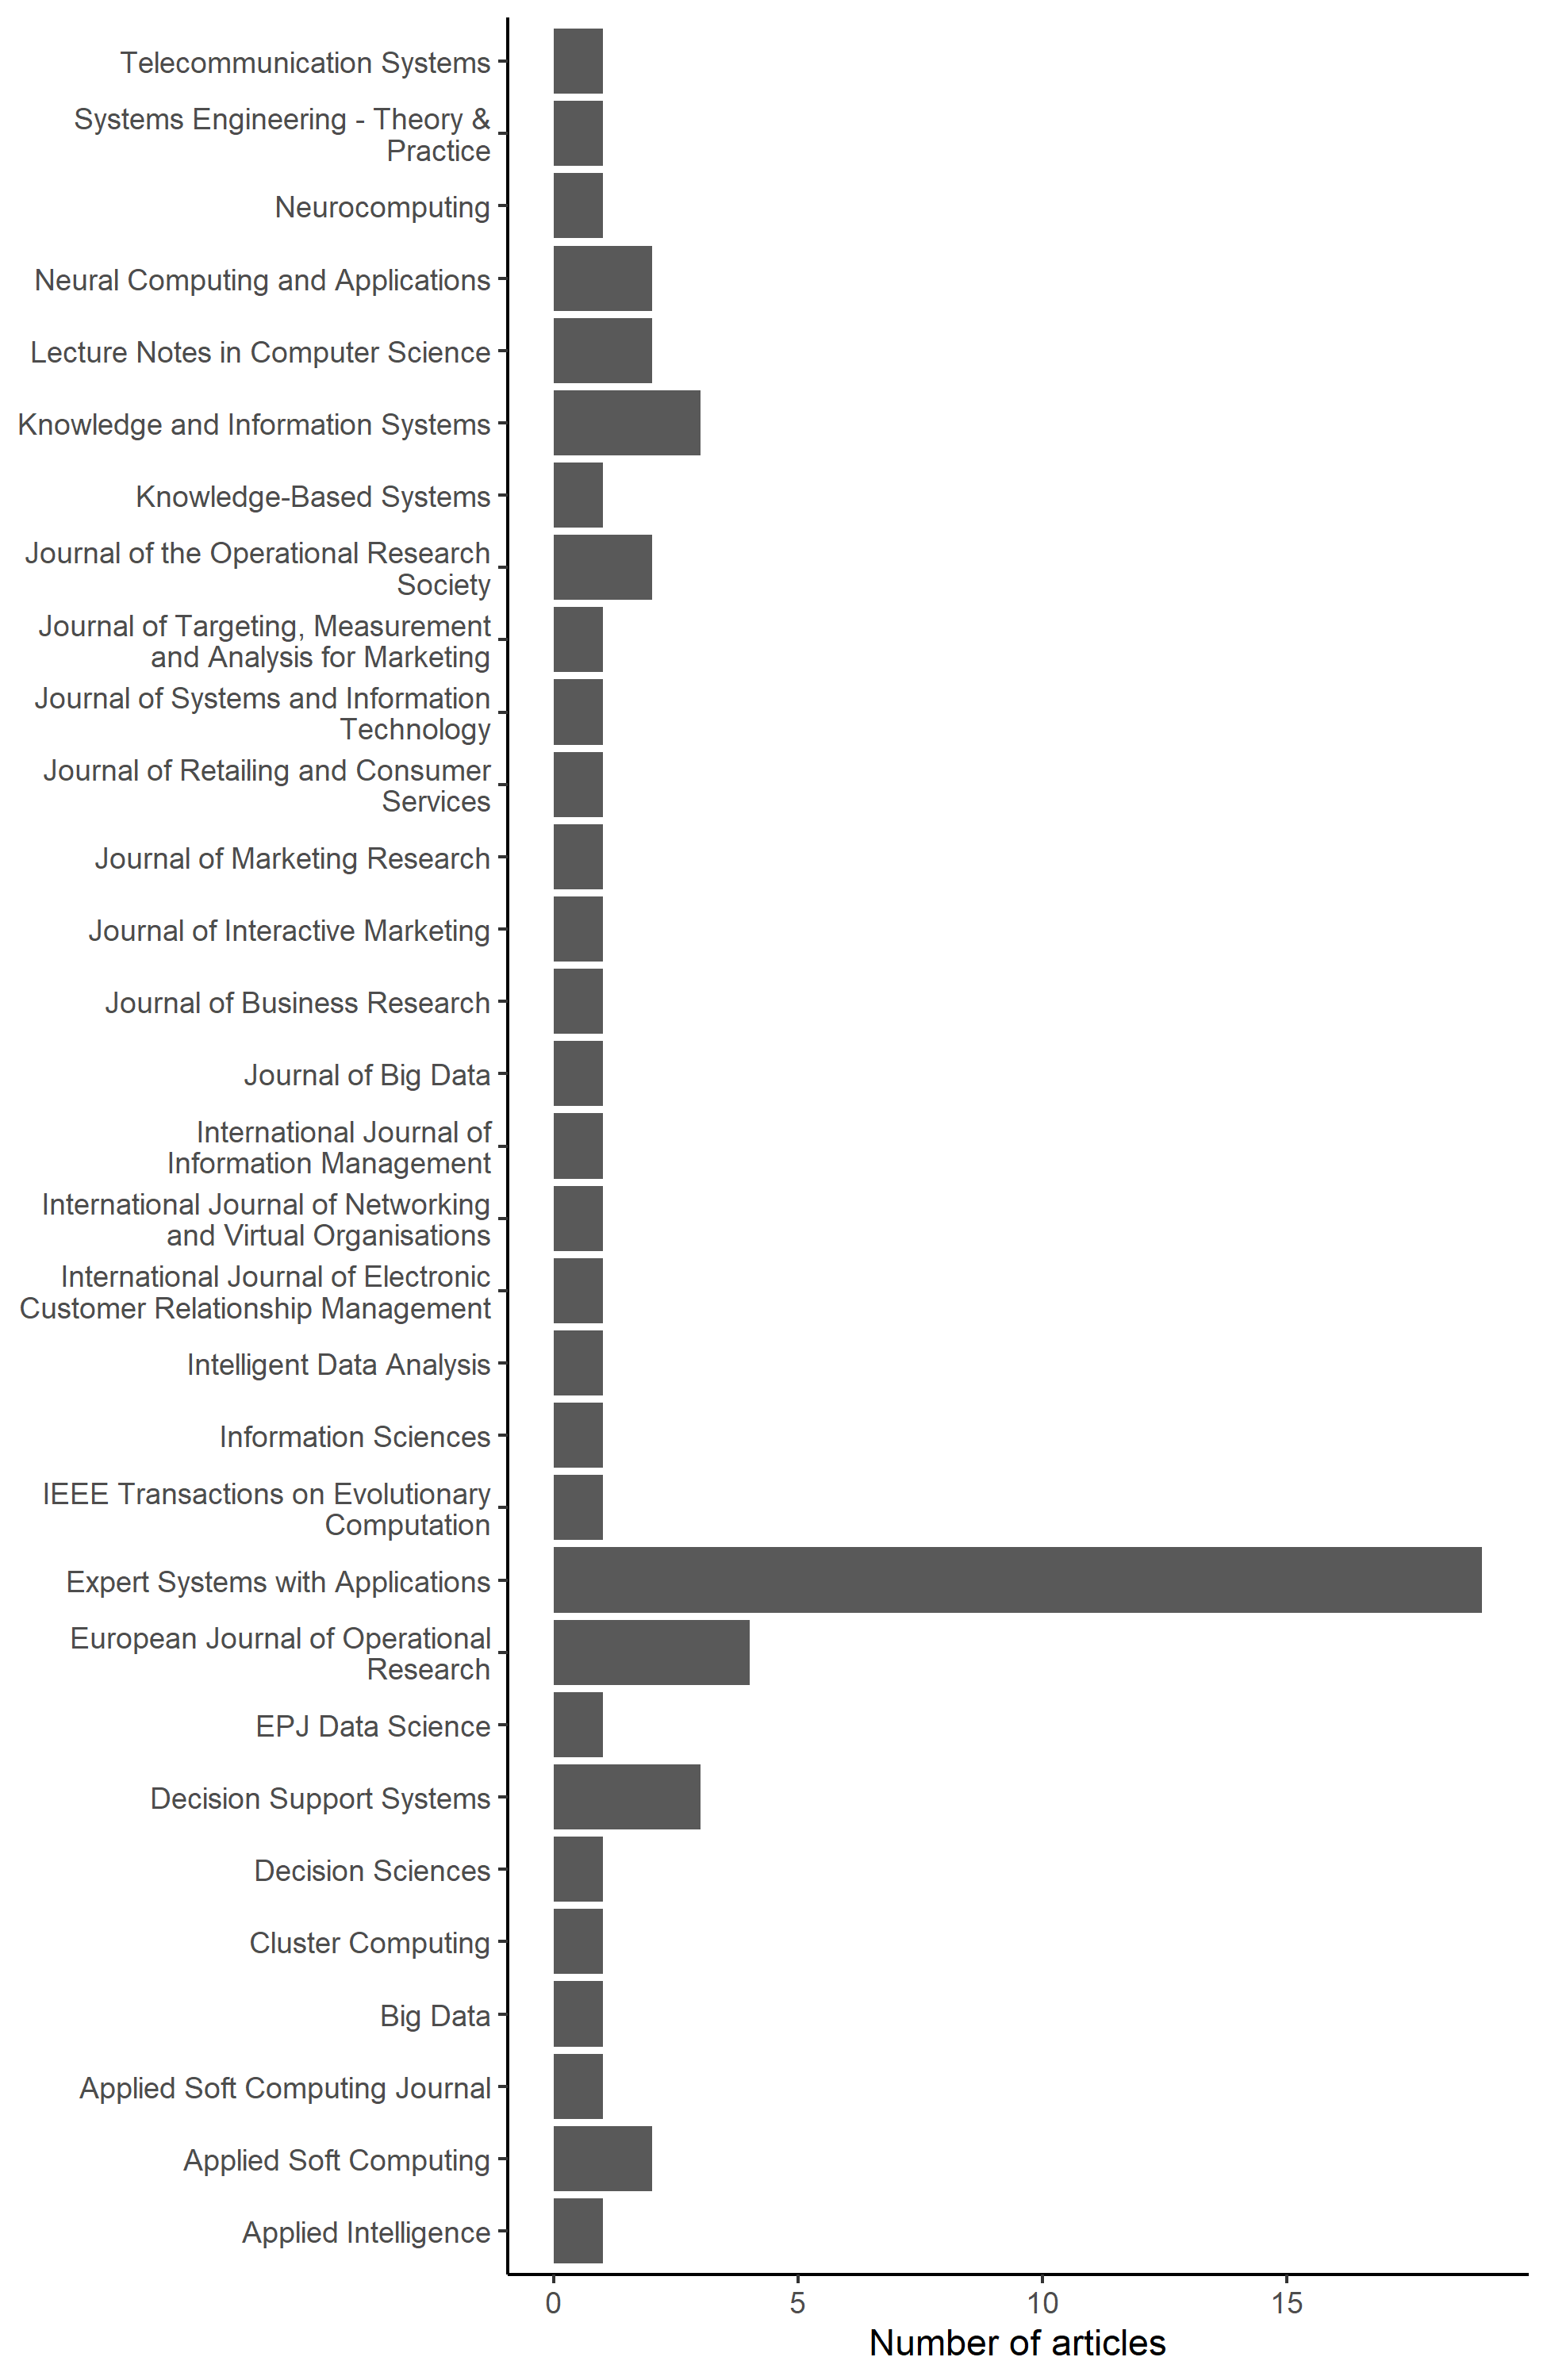
\includegraphics[width = 0.9\linewidth]{../figures/teste.png}
\begin{flushleft}
\end{flushleft}
\end{figure}
\vspace{-1.2cm}

\begin{Shaded}
\begin{Highlighting}[]
\CommentTok{\# Lets create a value for example}

\NormalTok{media }\OtherTok{\textless{}{-}} \FunctionTok{mean}\NormalTok{(cars}\SpecialCharTok{$}\NormalTok{speed)}
\end{Highlighting}
\end{Shaded}

The criminal rate is 15.4\%o.

\vspace{0.3cm}

\hypertarget{miguels-tests}{%
\section{Miguel's tests}\label{miguels-tests}}

\hypertarget{r}{%
\subsection{R}\label{r}}

Example of an equation

\[\int_0^{2\pi} \sin x~dx\]

\emph{Example of a matrix}

\[
\mathbf{X} = \left[\begin{array}
{rrr}
1 & 2 & 3 \\
4 & 5 & 6 \\
7 & 8 & 9
\end{array}\right]
\]

or

\begin{equation}
f\left(k\right) = \binom{n}{k}p^k\left(1-p\right)^{n-k} \label{eq:binom}
\end{equation}

See Equation \eqref{eq:binom}.

\begin{align}
y_{ijt} = \beta x_{ijt} + \eta_i + \gamma_j + \lambda_t + \varepsilon_{ijt}
\end{align}

\begin{Shaded}
\begin{Highlighting}[]
\FunctionTok{library}\NormalTok{(stargazer)}
\FunctionTok{stargazer}\NormalTok{(cars,}
          \AttributeTok{title =} \StringTok{"Summary 24"}\NormalTok{,}
          \AttributeTok{label =} \StringTok{"tab24"}\NormalTok{,}
          \AttributeTok{table.placement =} \StringTok{"ht"}\NormalTok{,}
          \AttributeTok{header =} \ConstantTok{FALSE}\NormalTok{)}
\end{Highlighting}
\end{Shaded}

\begin{table}[ht] \centering 
  \caption{Summary 24} 
  \label{tab24} 
\begin{tabular}{@{\extracolsep{5pt}}lccccccc} 
\\[-1.8ex]\hline 
\hline \\[-1.8ex] 
Statistic & \multicolumn{1}{c}{N} & \multicolumn{1}{c}{Mean} & \multicolumn{1}{c}{St. Dev.} & \multicolumn{1}{c}{Min} & \multicolumn{1}{c}{Pctl(25)} & \multicolumn{1}{c}{Pctl(75)} & \multicolumn{1}{c}{Max} \\ 
\hline \\[-1.8ex] 
speed & 50 & 15.400 & 5.288 & 4 & 12 & 19 & 25 \\ 
dist & 50 & 42.980 & 25.769 & 2 & 26 & 56 & 120 \\ 
\hline \\[-1.8ex] 
\end{tabular} 
\end{table}

\hypertarget{final-remarks}{%
\section{Final remarks}\label{final-remarks}}

Check the replication package for Bonhomme, Lamadon and Manresa (2019):
\url{https://github.com/tlamadon/blm-replicate}

\newpage

\hypertarget{references}{%
\section*{References}\label{references}}
\addcontentsline{toc}{section}{References}

\hypertarget{refs}{}
\begin{CSLReferences}{0}{0}
\end{CSLReferences}

\hypertarget{appendix-chunk-options}{%
\section*{Appendix: Chunk options}\label{appendix-chunk-options}}
\addcontentsline{toc}{section}{Appendix: Chunk options}

\hypertarget{software-versioning}{%
\subsection{Software versioning}\label{software-versioning}}

\hypertarget{r-1}{%
\subsubsection{R}\label{r-1}}

\begin{Shaded}
\begin{Highlighting}[]
\FunctionTok{cat}\NormalTok{(}\FunctionTok{paste}\NormalTok{(}\StringTok{"\#"}\NormalTok{, }\FunctionTok{capture.output}\NormalTok{(}\FunctionTok{sessionInfo}\NormalTok{()), }\StringTok{"}\SpecialCharTok{\textbackslash{}n}\StringTok{"}\NormalTok{, }\AttributeTok{collapse  =} \StringTok{""}\NormalTok{))}
\end{Highlighting}
\end{Shaded}

\begin{verbatim}
## # R version 4.1.0 (2021-05-18) 
## # Platform: x86_64-w64-mingw32/x64 (64-bit) 
## # Running under: Windows 10 x64 (build 19043) 
## #  
## # Matrix products: default 
## #  
## # locale: 
## # [1] LC_COLLATE=Portuguese_Portugal.1252  LC_CTYPE=Portuguese_Portugal.1252    
## # [3] LC_MONETARY=Portuguese_Portugal.1252 LC_NUMERIC=C                         
## # [5] LC_TIME=Portuguese_Portugal.1252     
## #  
## # attached base packages: 
## # [1] stats     graphics  grDevices utils     datasets  methods   base      
## #  
## # other attached packages: 
## #  [1] plotly_4.9.4.1   kableExtra_1.3.4 gtsummary_1.4.2  readxl_1.3.1     
## #  [5] stargazer_5.2.2  naniar_0.6.1     visdat_0.5.3     ggplot2_3.3.4    
## #  [9] dlookr_0.4.5     dplyr_1.0.7      
## #  
## # loaded via a namespace (and not attached): 
## #   [1] webshot_0.5.2       RColorBrewer_1.1-2  httr_1.4.2          
## #   [4] UpSetR_1.4.0        tools_4.1.0         backports_1.2.1     
## #   [7] utf8_1.2.1          R6_2.5.0            rpart_4.1-15        
## #  [10] lazyeval_0.2.2      Hmisc_4.5-0         nortest_1.0-4       
## #  [13] colorspace_2.0-1    nnet_7.3-16         withr_2.4.2         
## #  [16] tidyselect_1.1.1    gridExtra_2.3       curl_4.3.1          
## #  [19] compiler_4.1.0      extrafontdb_1.0     cli_2.5.0           
## #  [22] rvest_1.0.0         gt_0.3.0            htmlTable_2.2.1     
## #  [25] xml2_1.3.2          sandwich_3.0-1      labeling_0.4.2      
## #  [28] bookdown_0.22       scales_1.1.1        checkmate_2.0.0     
## #  [31] mvtnorm_1.1-2       proxy_0.4-26        RcmdrMisc_2.7-1     
## #  [34] systemfonts_1.0.2   stringr_1.4.0       digest_0.6.27       
## #  [37] foreign_0.8-81      rmarkdown_2.9       svglite_2.0.0       
## #  [40] rio_0.5.27          base64enc_0.1-3     jpeg_0.1-8.1        
## #  [43] pkgconfig_2.0.3     htmltools_0.5.1.1   extrafont_0.17      
## #  [46] highr_0.9           htmlwidgets_1.5.3   rlang_0.4.11        
## #  [49] rstudioapi_0.13     prettydoc_0.4.1     farver_2.1.0        
## #  [52] generics_0.1.0      jsonlite_1.7.2      zoo_1.8-9           
## #  [55] crosstalk_1.1.1     zip_2.2.0           car_3.0-11          
## #  [58] magrittr_2.0.1      Formula_1.2-4       Matrix_1.3-3        
## #  [61] Rcpp_1.0.6          munsell_0.5.0       fansi_0.5.0         
## #  [64] reticulate_1.20     abind_1.4-5         gdtools_0.2.3       
## #  [67] partykit_1.2-13     lifecycle_1.0.0     stringi_1.6.1       
## #  [70] yaml_2.2.1          inum_1.0-4          carData_3.0-4       
## #  [73] MASS_7.3-54         plyr_1.8.6          grid_4.1.0          
## #  [76] hrbrthemes_0.8.0    forcats_0.5.1       crayon_1.4.1        
## #  [79] lattice_0.20-44     haven_2.4.1         splines_4.1.0       
## #  [82] hms_1.1.0           knitr_1.33          pillar_1.6.1        
## #  [85] glue_1.4.2          evaluate_0.14       latticeExtra_0.6-29 
## #  [88] broom.helpers_1.3.0 data.table_1.14.0   png_0.1-7           
## #  [91] vctrs_0.3.8         Rttf2pt1_1.3.8      cellranger_1.1.0    
## #  [94] tidyr_1.1.3         gtable_0.3.0        purrr_0.3.4         
## #  [97] xfun_0.24           openxlsx_4.2.4      libcoin_1.0-8       
## # [100] e1071_1.7-7         class_7.3-19        survival_3.2-11     
## # [103] viridisLite_0.4.0   tibble_3.1.2        cluster_2.1.2       
## # [106] corrplot_0.89       ellipsis_0.3.2
\end{verbatim}

\begin{Shaded}
\begin{Highlighting}[]
  \CommentTok{\# or use message() instead of cat()}
\end{Highlighting}
\end{Shaded}


\end{document}
